\documentclass[10pt]{beamer}
\setbeamertemplate{caption}[numbered]
\usepackage[utf8]{inputenc}
\usepackage[french]{babel}
\usepackage{amsmath}
\usepackage{graphicx}
\usepackage{stmaryrd}
\usepackage{bbm}
\usepackage{listings}
\usepackage[section]{placeins}
\usepackage{caption}
\usepackage{url}

\usetheme{Malmoe}

\usepackage{color} %red, green, blue, yellow, cyan, magenta, black, white
\definecolor{mygreen}{RGB}{28,140,0} % color values Red, Green, Blue
\definecolor{mylilas}{RGB}{170,55,241}

\lstset{language=Matlab,%
    %basicstyle=\color{red},
    basicstyle= \ttfamily \footnotesize,
    breaklines=true,%
    morekeywords={matlab2tikz},
    keywordstyle=\color{blue},%
    morekeywords=[2]{1}, keywordstyle=[2]{\color{black}},
    identifierstyle=\color{black},%
    stringstyle=\color{mylilas},
    commentstyle=\color{mygreen},%
    showstringspaces=false,%without this there will be a symbol in the places where there is a space
    %numbers=left,%
    numberstyle={\tiny \color{black}},% size of the numbers
    numbersep=9pt, % this defines how far the numbers are from the text
    emph=[1]{for,end,break},emphstyle=[1]\color{red}, %some words to emphasise
    %emph=[2]{word1,word2}, emphstyle=[2]{style}, 
    frame = single
}



\title{Méthodes à haute résolution}
\author{Augustin HOFF et Gustavo CIOTTO PINTON}
\institute{ 
\includegraphics[scale=0.1]{images/LogoSupelec}}
\date{2014}


\begin{document}

    \begin{frame}
    \titlepage
    \end{frame}
    
    \begin{frame}
    \frametitle{Table des matières }
    \tableofcontents
    \end{frame}

    \section{Généralités}
    \subsection{Outils mathématiques} 
    
    % ----------------------%%%%%%%%%%%
    
    \begin{frame}
    
        \frametitle{Outils mathématiques}
        \framesubtitle{Définitions}
        \begin{itemize}
        \item L'autocorrelation d'un processus aléatoire pour deux indices de temps différents \(n_1\) et \(n_2\) est définie comme
        \begin{equation}
        %
            \label{eq:autocorr} 
            r_{xx} = \mathcal E \{ x[n_1]x^*[n_2] \}
        %
        \end{equation}
        
        
        \item La matrice formée par les valeurs d'autocorrelation:

         { \fontsize{8.5}{10}\selectfont

        \begin{equation}
        %
            \label{eq:matricecorr}
            R_{N-1}=\begin{bmatrix}
                r_{xx}[0] & r_{xx}[-1] & r_{xx}[-2] & \cdots & r_{xx}[-(N-1)] \\
                r_{xx}[1] & r_{xx}[0] & r_{xx}[-1] & \cdots & r_{xx}[-(N-2)] \\
                \vdots & \vdots & \vdots & \ddots & \vdots \\
                r_{xx}[N-1] & r_{xx}[N-2] & r_{xx}[N-3] & \cdots & r_{xx}[0] \\
            \end{bmatrix}
        %
        \end{equation}
        }
        
        \end{itemize}
    \end{frame}
    
    
    % ----------------------%%%%%%%%%%%
    
    \begin{frame}
    
        \frametitle{Outils mathématiques}
        \framesubtitle{Définitions}
        
        \begin{itemize}
        
        \item Le rapport entre les puissances du signal et du bruit (SNR):
        
        \begin{equation}
            SNR = \frac{P_{signal}}{P_{bruit}}
        \end{equation}
        
        Il est souvent écrit en \textit{décibels} [dB]:
        
        \begin{equation}
            \label{eq:snr}
            SNR_{dB} = 10* \log \left[ \frac{P_{signal}}{P_{bruit}} \right]
        \end{equation}
        
        \item La puissance d'un processus aléatoire est calculée par l'équation suivante
        
        \begin{equation}
            P_x = \frac{1}{2\pi} \int_{-\pi}^{\pi}  S_x (\omega) d\omega = \int_{-\frac{1}{2}}^{\frac{1}{2}}  S_x (\nu) d\nu
        \end{equation}
        
        où \(S_x(f) = \mathcal{F} \{r_{xx}[k]\}\)
        
        \end{itemize}
    \end{frame}
    
    
    % ----------------------%%%%%%%%%%%


    \subsection{Application à un signal sinuisoïdal complexe} 
    \begin{frame}
    
        \frametitle{Outils mathématiques}
        \framesubtitle{Application à un signal sinuisoïdal complexe}
        
        \begin{itemize}
        
        \item On pose le signal d'entrée
        
        \begin{equation}
        \label{eq:x}
            s[n] = \sum_{k=1}^{P} A_k \exp(j(2\pi f_k n T + \theta _k))
        \end{equation}
        
        \item 
        
        En supposant que les variables aléatoires \(\theta _k\) sont idépendantes et uniformement distribuées sur l'intervalle \( [0, 2\pi[\), on obtient alors
        
        \begin{equation}
        \label{eq:meanx}
            \overline{s}[n] = 0 \text{ \hspace{5pt} et \hspace{5pt} } r_{ss}[m] = \sum_{k=1}^{P} A_k^2 \exp(j 2\pi f_k m T)
        \end{equation}
        
        De plus:
        
        \begin{equation}
        SNR_{dB} = 10* \log \left[ \frac{P_{signal}}{P_{bruit}} \right] = 10* \log \left[ \frac{\sum_{k=1}^{P}A_k^2}{P_{bruit}} \right]
        \end{equation}
        
        \end{itemize}
    \end{frame}
    
    
    % ----------------------%%%%%%%%%%%
    
        \begin{frame}
    
        \frametitle{Outils mathématiques}
        \framesubtitle{Application à un signal sinuisoïdal complexe}
        
        \begin{itemize}
        
        \item La matrice d'autocorrelation s'écrit en présence de bruit blanc de variance \(p_w\) 

        \begin{equation}
        %
            \label{eq:Ryy}
            R_{xx}= R_{ss} + R_w =\sum_{k=1}^{P}A_k^2 \boldsymbol{e}_{N-1}(f_k) \boldsymbol{e}_{N-1}^H(f_k) + p_w\boldsymbol{I}
        %
        \end{equation}
        
        où 

        \begin{equation}
        %
            \label{eq:em}
            \boldsymbol{e}_{N-1}(f_k)=\begin{bmatrix}
                1 \\
                \exp (2 \pi j f_k T) \\
                \vdots \\
                \exp (2 \pi j f_k (N-1)T) \\
            \end{bmatrix}
        %
        \end{equation}
        
                
        \end{itemize}
    \end{frame}
        
    % ----------------------%%%%%%%%%%%
    
        \begin{frame}
    
        \frametitle{Outils mathématiques}
        \framesubtitle{Application à un signal sinuisoïdal complexe}
        
        \begin{itemize}        
        \item La matrice se réécrit à partir des P valeurs propres de \(R_{ss}\)
        
        \begin{equation}
%
        \label{eq:RyyEigen}
        R_{xx} = \sum_{i=1}^{P}(\lambda _i + p_w) \boldsymbol{v}_{i} \boldsymbol{v}_{i}^H + p_w\sum_{i=P+1}^{N} \boldsymbol{v}_{i} \boldsymbol{v}_{i}^H
%
        \end{equation} 
        
        \item Les P premiers vecteurs propres de \(R_{xx}\) forment l'espace signal \underline {orthogonal} à l'espace bruit donné par les N-P autres vecteurs propres. 
        
        \end{itemize}
    \end{frame}
    
    
    % ----------------------%%%%%%%%%%%

    \section{Algorithme MUSIC}
    \subsection{Aspect théorique} 
    
    % ----------------------%%%%%%%%%%%

    \begin{frame}
    
        \frametitle{Algorithme MUSIC}
        \framesubtitle{Aspect théorique}
        
        \begin{itemize}
        
        \item On pose alors:
        
        { \fontsize{8.5}{10}\selectfont
        
        \begin{equation}
%
        \label{eq:basemusic}
        \sum_{k=P+1}^{N} \alpha _k \left| \boldsymbol{e}_{N-1}^H (f) \boldsymbol{v}_k \right| ^2 = \boldsymbol{e}_{N-1}^H (f) \left( \sum_{k=P+1}^{N} \alpha _k  \boldsymbol{v}_{k}\boldsymbol{v}_k^H \right) \boldsymbol{e}_{N-1} (f)
%
        \end{equation}
        }
        
        \item Cette quantité est nulle si \(\boldsymbol{e}_{N-1}(f)\) est un des vecteurs de l'espace signal i.e si f est une fréquence du signal car \(\boldsymbol{v}_k \) est un vecteur propre de l'espace bruit pour k \( \in \llbracket P+1,N \rrbracket \)
        
        \item L'estimateur est donc donné par l'expression

        \begin{equation}
        %
            \label{eq:music}
            P_{MUSIC} (f) = \frac{1}{\boldsymbol{e}_{N-1}^H (f) \left( \sum_{k=P+1}^{N}   \boldsymbol{v}_{k}\boldsymbol{v}_k^H \right) \boldsymbol{e}_{N-1} (f)}
        %
        \end{equation}
        
        \end{itemize}
    \end{frame}
    
    
    % ----------------------%%%%%%%%%%%





    \subsection{Mise en oeuvre} 
    
    % ----------------------%%%%%%%%%%%
    
    \begin{frame}[fragile]
    %
        \frametitle{Algorithme MUSIC}
        \framesubtitle{Mise en oeuvre - \textit{P\_music.m}}
%       
%       
        \begin{itemize}
        \item  Les principales variables
        
        \begin{lstlisting}
function [ resultat ] = P_music(signal_x,  frequences , P)
N = size(signal_x ,2);
T = 1/N;
        \end{lstlisting}
%        
        \item  Calcul de la matrice d'autocorrelation  
        
        \begin{lstlisting}
z   = corrmtx( signal_x, 0 );
Rxx = toeplitz(z);
        \end{lstlisting} 

        \end{itemize}
\end{frame}


    % ----------------------%%%%%%%%%%%
    
    \begin{frame}[fragile]
    %
        \frametitle{Algorithme MUSIC}
        \framesubtitle{Mise en oeuvre - \textit{test.m}}
%       
%       
        \begin{itemize}

        \item Paramètres initiaux du test
        
        \begin{lstlisting}
clear all; close all; clc;
N = 100;
n = 0: 1 : N - 1;
P = 3;
T = 1/N;            
fDebut = 1e0;
fFin   = 7e1;       
fPas   = 1e-1; 

A = [1 2.5 3];
F = [4.9e1 5e1 6e1];
Theta = 2*pi*[rand(1) rand(1) rand(1)];

SNR = [0.001 40 100 500]; %(dB)

        \end{lstlisting} 
        
        \end{itemize}
\end{frame}


    % ----------------------%%%%%%%%%%%
    
    \begin{frame}[fragile]
    %
        \frametitle{Algorithme MUSIC}
        \framesubtitle{Mise en oeuvre - \textit{test.m}}
%       
%       
        \begin{itemize}

        \item Calcul des pics pour chaqu'un des SNRs
        
        \begin{lstlisting}
bAux = randn(1,N);

%signal
s = zeros (1, N); 
for k = 1:P
    s = s + A(k) * exp(2*pi*1i*n*T*F(k) + 1i*Theta(k));
end

%bruit
for l = 1 : size(SNR, 2)

    varianceNoise = sum (A.*A) / ( 10 ^ (SNR(l) / 10));
    b = sqrt(varianceNoise) * bAux;
    x = s + b;
    
    frequences = fDebut : fPas : fFin;
    result = P_music (x, frequences, P);
    plot(...)
end
        \end{lstlisting} 
        
        \end{itemize}
\end{frame}


    % ----------------------%%%%%%%%%%%
    
    \subsection{Resultats} 
    
    \begin{frame}
    %
        \frametitle{Algorithme MUSIC}
        \framesubtitle{Resultats}
        
        \begin{figure}[h]
            \centering
            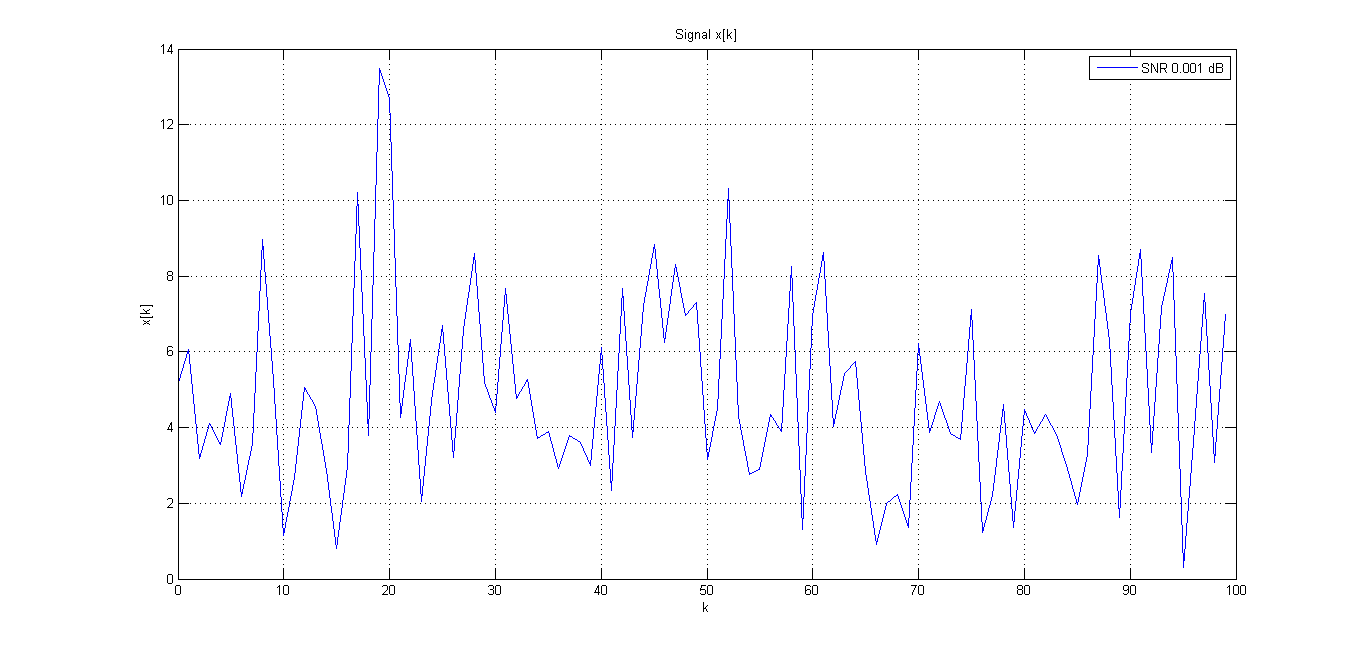
\includegraphics[scale= 0.28 ]{images/wave0001}
            \caption{Signal avec du bruit pour \(SNR_{dB} = 0.001 dB\)}
            \label{fig:snr0001}
        \end{figure}
        
    \end{frame}
    
    % ----------------------%%%%%%%%%%%
    
    \begin{frame}
    %
        \frametitle{Algorithme MUSIC}
        \framesubtitle{Resultats}
        
        \begin{figure}[h]
            \centering
            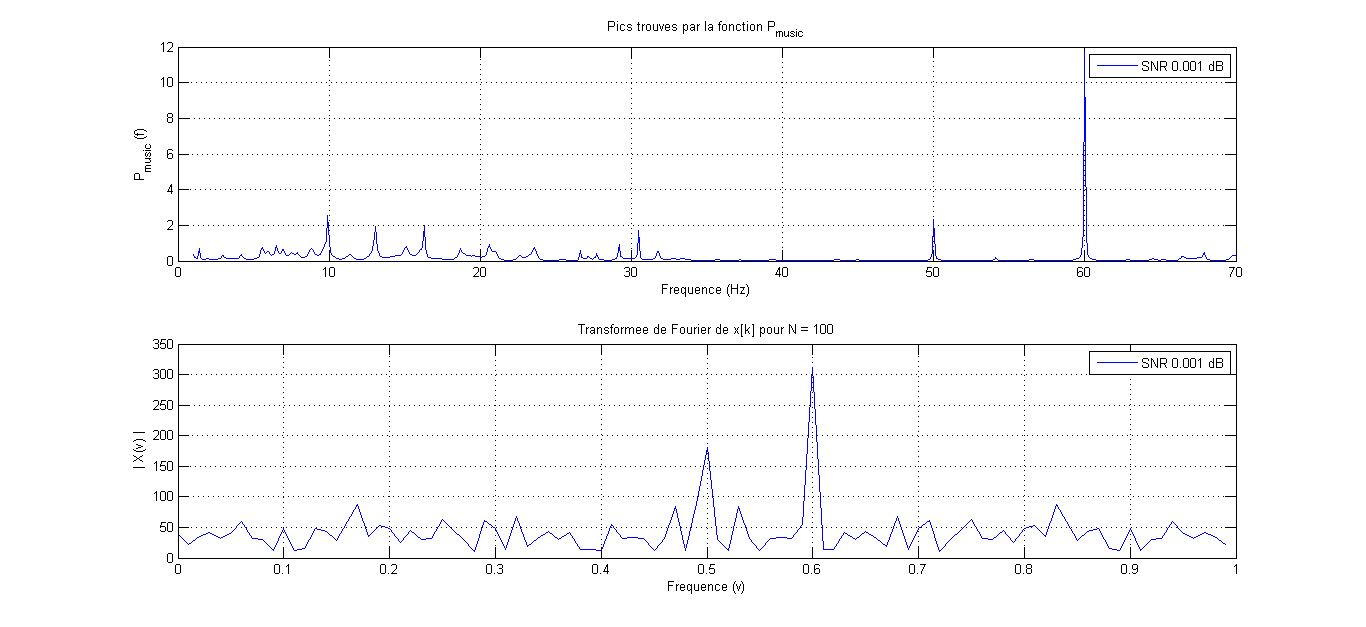
\includegraphics[scale= 0.28]{images/snr0001}
            \caption{Resultats obtenus pour \(SNR_{dB} = 0.001 dB\)}
            \label{fig:wave0001}
        \end{figure}
        
    \end{frame}
    
    % ----------------------%%%%%%%%%%%
    
    \begin{frame}
    %
        \frametitle{Algorithme MUSIC}
        \framesubtitle{Resultats}
        
        \begin{figure}[h]
        %
            \centering
            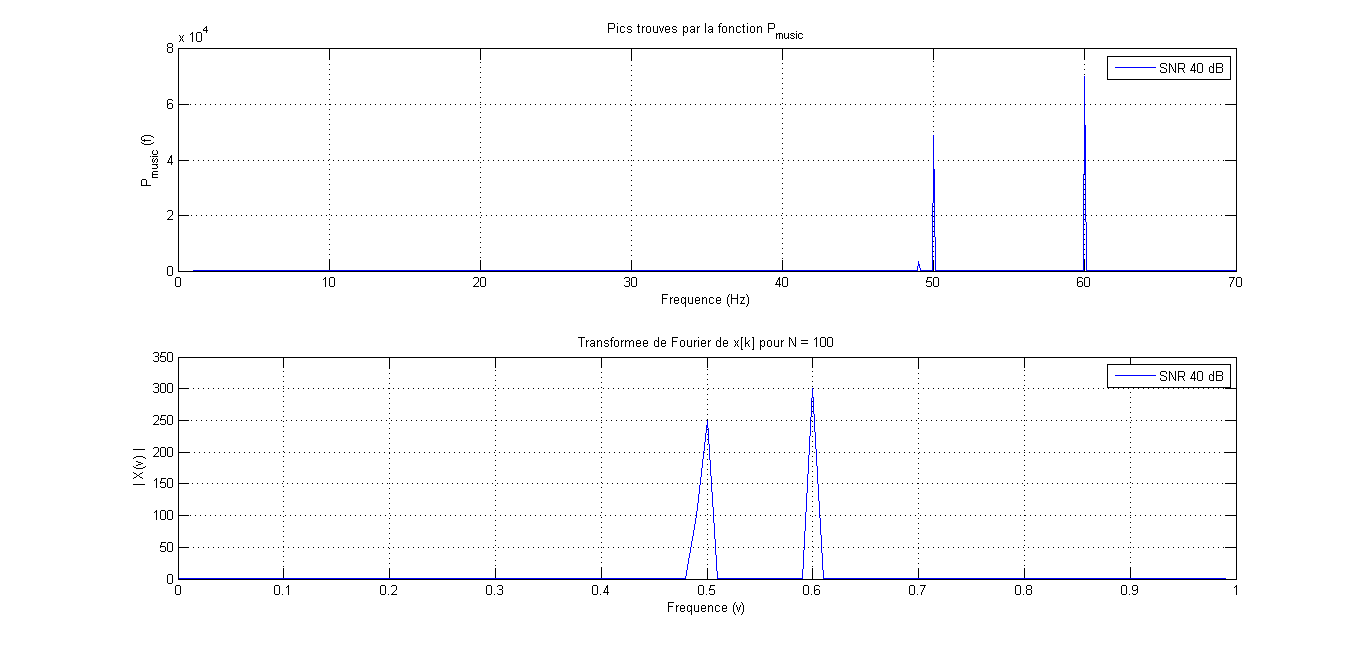
\includegraphics[scale=0.28 ]{images/snr40}
            \caption{Resultats obtenus pour \(SNR_{dB} = 40 dB\)}
            \label{fig:snr40}
        \end{figure}
    \end{frame}
    
    % ----------------------%%%%%%%%%%%    
        
    \begin{frame}
    %
        \frametitle{Algorithme MUSIC}
        \framesubtitle{Resultats}
        
        \begin{figure}[h]
            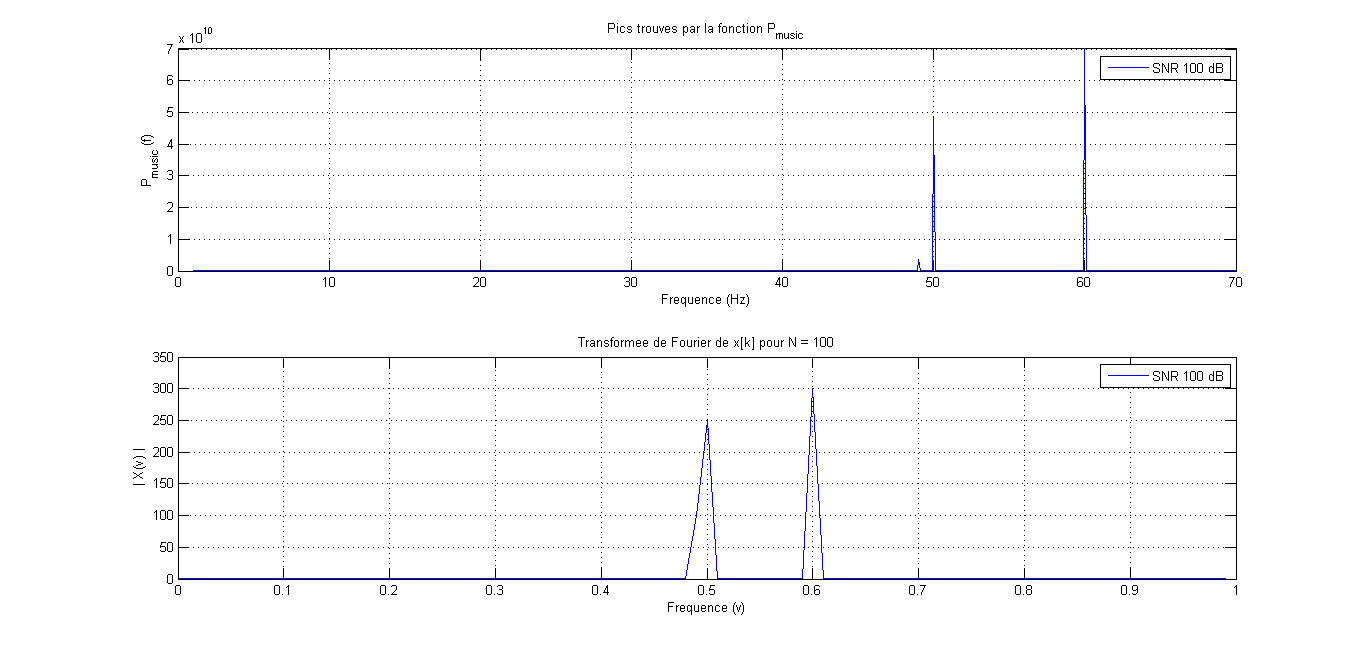
\includegraphics[scale=0.28 ]{images/snr100}
            \caption{Resultats obtenus pour \(SNR_{dB} = 100 dB\)}
            \label{fig:snr100}
        \end{figure}
        
    \end{frame}
    
    % ----------------------%%%%%%%%%%%
    
    \begin{frame}
    %
        \frametitle{Algorithme MUSIC}
        \framesubtitle{Resultats}
        
        \begin{figure}[h]
            \centering
            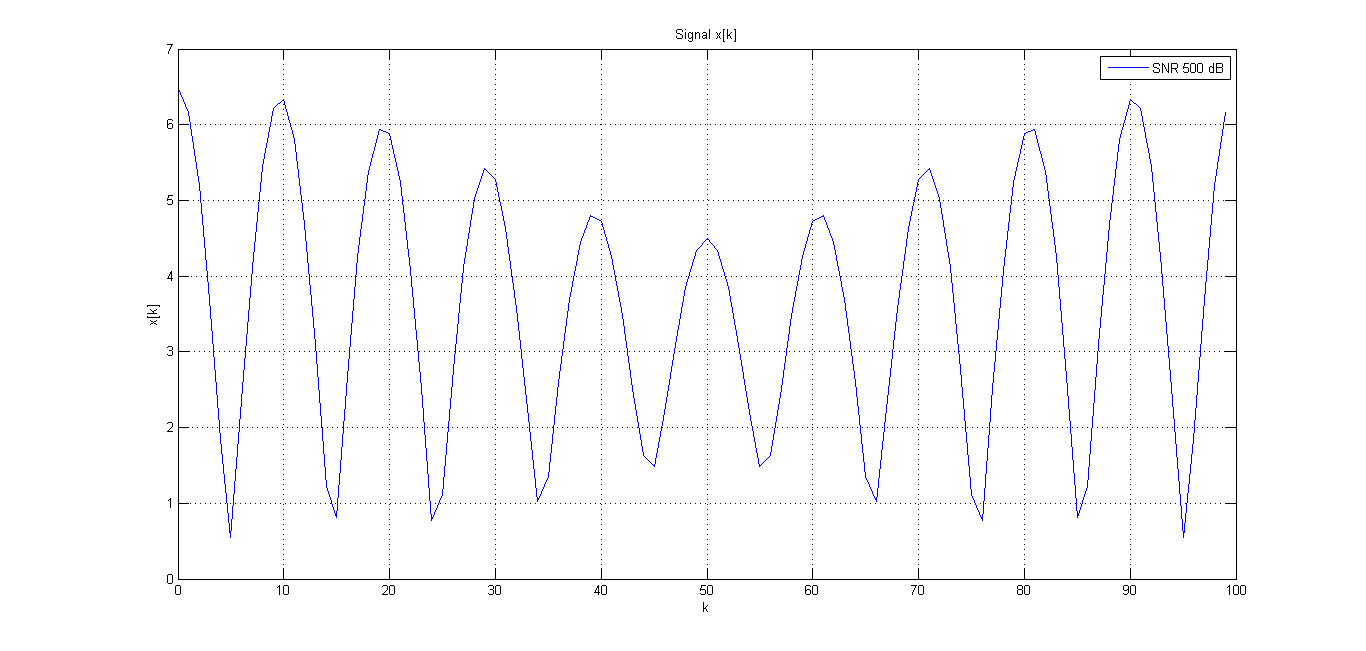
\includegraphics[scale= 0.28 ]{images/wave500}
            \caption{Signal avec du bruit pour \(SNR_{dB} = 500 dB\)}
            \label{fig:snr0001}
        \end{figure}
        
    \end{frame}
    
    % ----------------------%%%%%%%%%%%
    
    \begin{frame}
    %
        \frametitle{Algorithme MUSIC}
        \framesubtitle{Resultats}
        
        \begin{figure}[h]
            \centering
            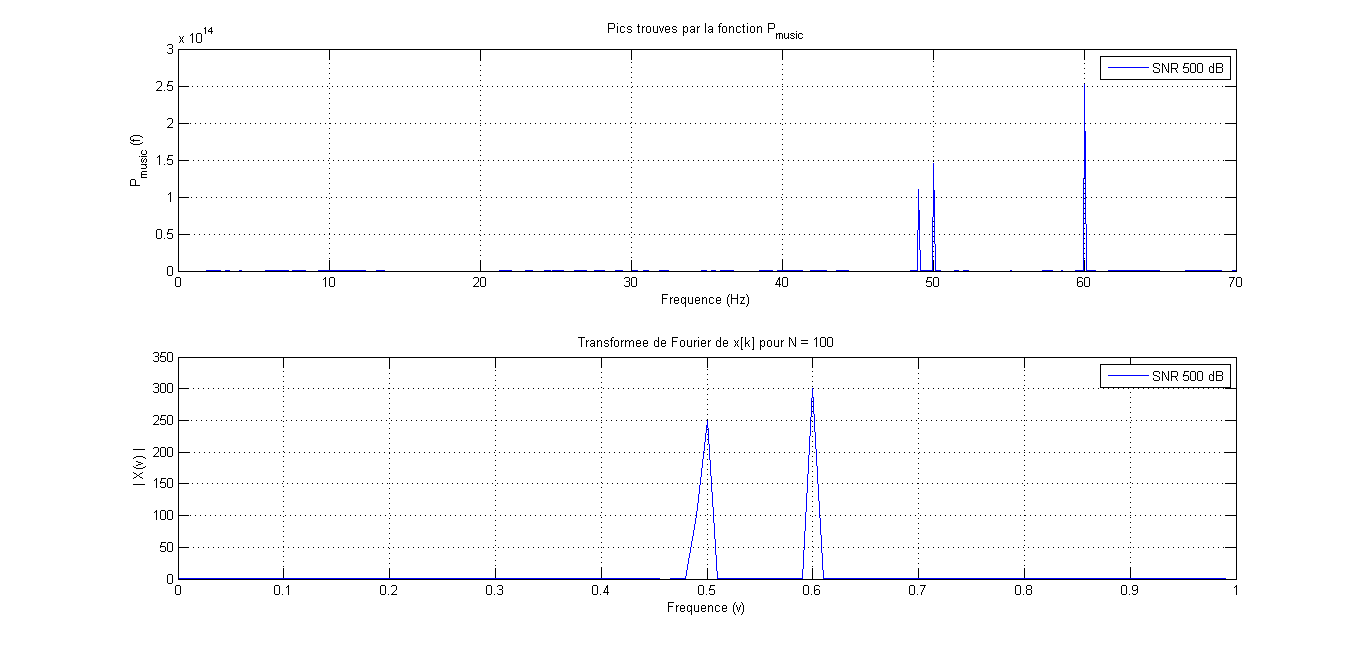
\includegraphics[scale= 0.28]{images/snr500}
            \caption{Resultats obtenus pour \(SNR_{dB} = 500 dB\)}
            \label{fig:wave500}
        \end{figure}
        
    \end{frame}
    
    % ----------------------%%%%%%%%%%%

    \subsection{Critère de Rayleight}    
    \begin{frame}
    %
        \frametitle{Critère de Rayleight}
        \framesubtitle{Analogie avec la lumière}
        
        \begin{figure}[h]
            \centering
            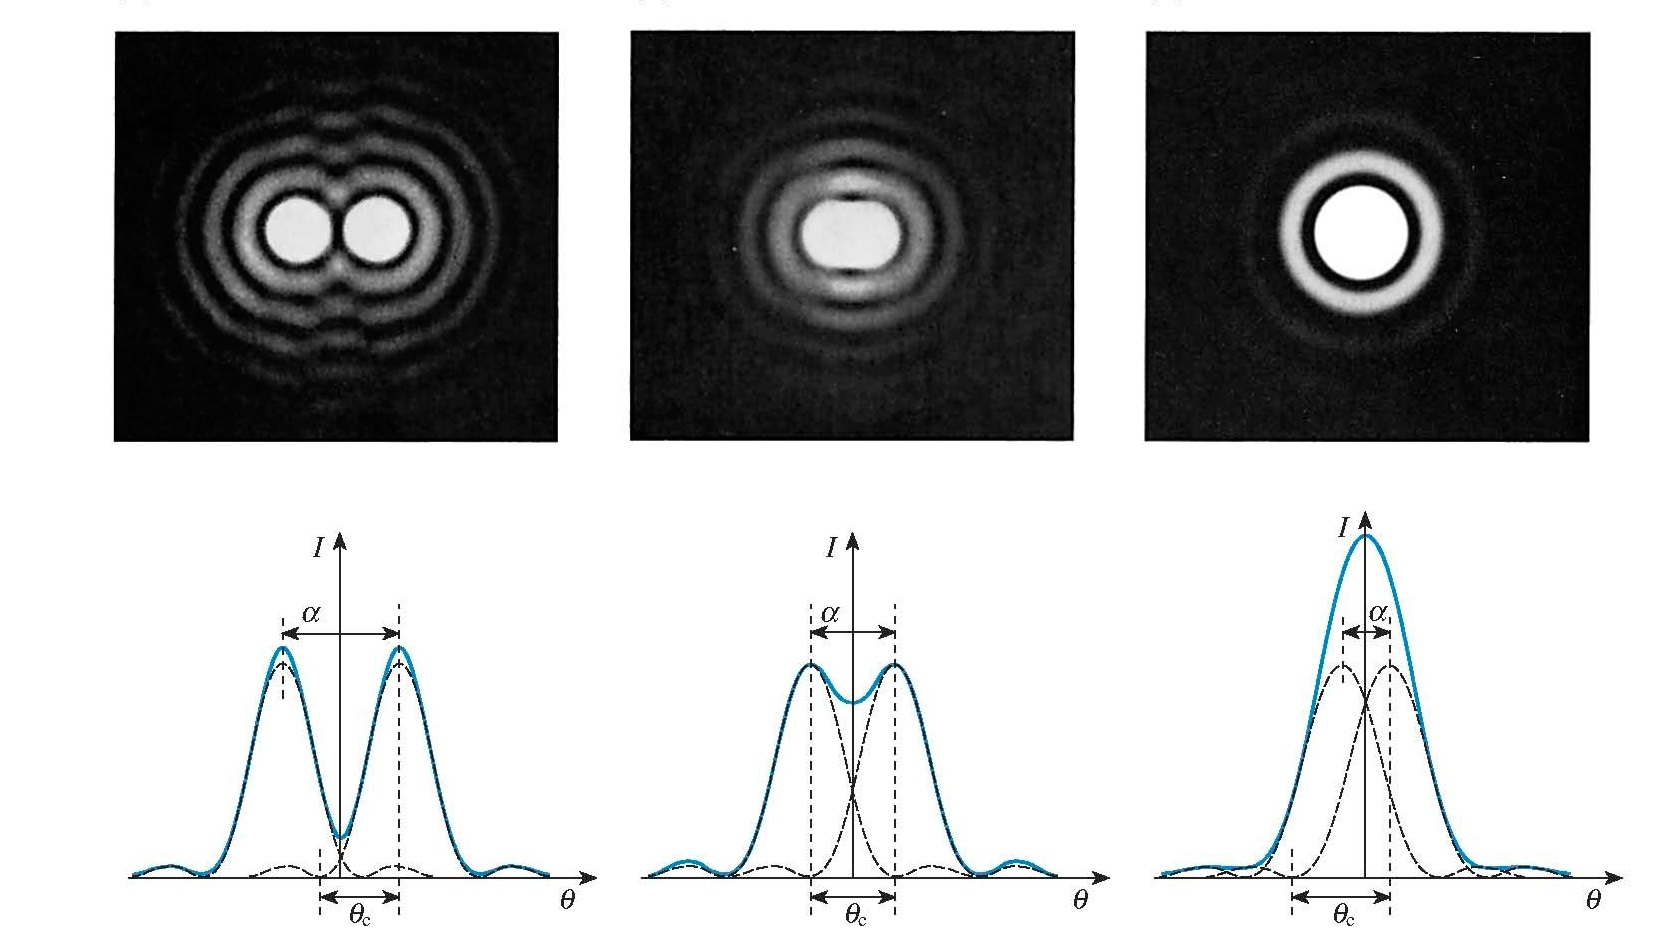
\includegraphics[scale= 0.22]{images/Critere_Rayleight2}
            \caption{Distinction des différentes taches de lumière selon les cas}
        \end{figure}

    \end{frame}
    
    % ----------------------%%%%%%%%%%%
    
    \section{Algorithme ESPRIT}    
    \begin{frame}
    %
        \frametitle{Algorithme ESPRIT}
        
        \begin{figure}[h]
            \centering
            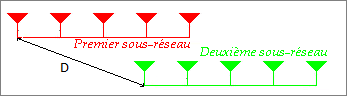
\includegraphics[scale=.6]{images/ReseauEsprit}
            \caption{Disposition des antennes.}
        \end{figure}
        
        Déphasage temporel de \( \frac{D sin(\phi) }{c}  \) où
        \(\phi\) est l'angle d'incidence du signal

        
    \end{frame}
    
    % ----------------------%%%%%%%%%%%
    
    \begin{frame}
    %
        \frametitle{Algorithme ESPRIT}
        
        \begin{equation}
          S_2 = S_1 \Omega
        \end{equation}
        
        si \[ S_1 = \begin{bmatrix}
        \boldsymbol{e}_{N-1}(f_1) & \cdots & \boldsymbol{e}_{N-1}(f_P)
    \end{bmatrix} \]
    
    et \[ \Omega = \begin{bmatrix}
         \exp(2\pi j f_1 \frac{D sin(\phi_1) }{c}) & & \text{\huge0}\\
         &  \ddots \\
         \text{\huge0} & & \exp(2\pi j f_p \frac{D sin(\phi_P) }{c})\\

         \end{bmatrix} \]

    \end{frame}
    
    % ----------------------%%%%%%%%%%%
    
    \begin{frame}
    %
        \frametitle{Algorithme ESPRIT}
         \begin{itemize}

        \item La matrice d'autocorrélation s'écrit alors 
\begin{equation}
R_{xx} = \begin{bmatrix} S_1 \\ S_1 \Omega \end{bmatrix} 
\begin{bmatrix} A_1^2 & & \text{0}\\ &  \ddots \\ \text{0} & & A_P^2 \\ \end{bmatrix}
\begin{bmatrix}   S_1 \\ S_1 \Omega \end{bmatrix}^H  + p_w\boldsymbol{I}
\end{equation}

        \item Ce qui donne:
        \begin{equation}
U = [u_1 \cdots u_P] = \begin{bmatrix} U_1 \\ U_2 \end{bmatrix} = \begin{bmatrix} S_1 \\ S_1 \Omega \end{bmatrix} T = \begin{bmatrix} S_1 T \\ S_1 \Omega T \end{bmatrix}
\end{equation}
\end{itemize}

    \end{frame}
    
     % ----------------------%%%%%%%%%%%
    
    \begin{frame}
    %
        \frametitle{Algorithme ESPRIT}
         \begin{itemize}

\item Finalement 
\begin{equation}
U_2 = U_1 T^{-1} \Omega T = U_1 \Psi
\end{equation}

\item La méthode des moindres carrés donne alors une estimation de \( \Psi\) la matrice semblable à \( \Omega\) contenant les informations du signal

\begin{equation}
\Psi = (U_1 U_1^H)^{-1} U_1^H U_2
\end{equation}
      
\end{itemize}

    \end{frame}
    
    % ----------------------%%%%%%%%%%%
    
    \section {Références}
    \begin{frame}{Références}
    
        \begin{itemize}
        \item 
        Institute for Dynamics Systems and Control. \textit{White noise and power spectral density}.\\
        \url{http://www.idsc.ethz.ch/Courses/signals_and_systems/ArchiveFall10/lectureNotes8.pdf}
        
        \item S. Lawrence Marple Jr. \textit{Digital Spectral Analysis with Applications}. Prentice-Hall Inc, 1988
        
        \item Bernard Picinbono. \textit{Signaux aléatoires - Tome 2 Fonctions aléatoires et modèles avec problèmes résolus}. Dunod Université, 1993
        
        \item \textit{Les méthodes à haute résolution}. HERMES, 1998
        
        \item Yves Grenier. \textit{Méthodes haute-résolution en analyse spectrale et localisation}. \\
\url{http://perso.telecom-paristech.fr/~rioul/liesse/2012liesse4/YG-slides.pdf}
        
        \end{itemize}

    \end{frame}
    
\end{document}